\chapter{Hello World!}

\section{Hello World!}

\subsection{编程语言(Programming Language)}

程序是为了让计算机去解决某些问题,它由一系列指令构成。但是计算机并不能理解人类的语言,即使是最简单的,例如“计算一下1+2是多少”。\\

计算机采用的是二进制(binary),也就是只能够理解0和1,因此编程语言用于作为人类与计算机之间沟通的桥梁。

\begin{figure}[H]
	\centering
	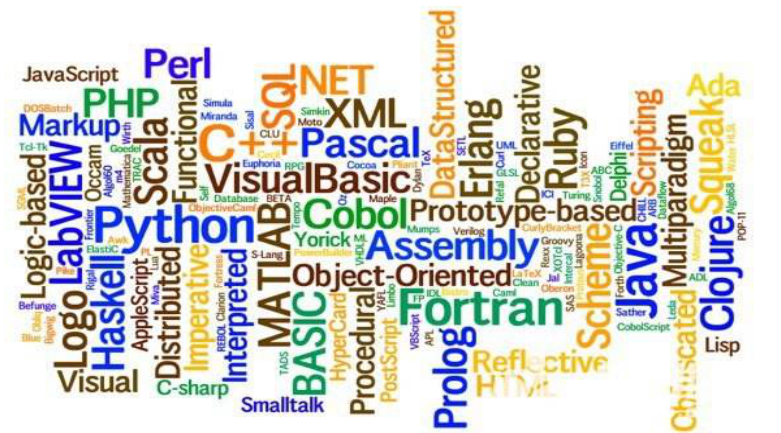
\includegraphics[scale=0.9]{img/Chapter1/1-1/1.png}
\end{figure}

通过使用编程语言来描述解决问题的步骤,从而让计算机一步一步去执行。流程图(flow chat)成为了一种程序的图形化表示方式。\\

\begin{figure}[H]
	\centering
	\begin{tikzpicture}[node distance=2cm]
		\node (start) [startend] {Start};
		\node (init) [io, below of=start] {$ i = 0 $, $ sum = 0 $};
		\node (decision)  [decision, below of=init] {$ i \le 100 $?};
		\node (accumulation) [process, below of=decision] {$ sum = sum + i $};
		\node (update) [process, below of=accumulation] {$ i = i + 1 $};
		\node (output) [io, right of=decision, xshift=2.5cm] {print $ sum $};
		\node (end) [startend, below of=update] {End};

		\draw [arrow] (start) -- (init);
		\draw [arrow] (init) -- (decision);
		\draw [arrow] (decision) -- node[anchor=east] {yes } (accumulation);
		\draw [arrow] (accumulation) -- (update);
		\draw [arrow] (update) -- (-3,-8) -- (-3,-4) -- (decision);
		\draw [arrow] (decision) -- node[anchor=south] {no} (output);
		\draw [arrow] (output) |- (end);
	\end{tikzpicture}
	\caption{计算$ \sum_{i=1}^{100} i $的流程图}
\end{figure}

\vspace{0.5cm}

\subsection{Hello World!}

Hello World是学习编程的第一个程序,它的作用是向屏幕输出"Hello World!"。\\

\mybox{Hello World!}

\begin{lstlisting}[language=Python]
print("Hello World!")
\end{lstlisting}

\begin{tcolorbox}
	\mybox{运行结果}
	\begin{verbatim}
Hello World!
	\end{verbatim}
\end{tcolorbox}

不同编程语言的Hello World写法大同小异,可以看出编程语言的基本结构是相似的。\\

\mybox{C}

\begin{lstlisting}[language=C]
#include <stdio.h>

int main() {
	printf("Hello World!\n");
	return 0;
}
\end{lstlisting}

\vspace{0.5cm}

\mybox{C++}

\begin{lstlisting}[language=C++]
#include <iostream>

using namespace std;

int main() {
	cout << "Hello World!" << endl;
	return 0;
}
\end{lstlisting}

\vspace{0.5cm}

\mybox{Java}

\begin{lstlisting}[language=Java]
public class HelloWorld {
    public static void main(String[] args) {
        System.out.println("Hello World!");
    }
}
\end{lstlisting}

\vspace{0.5cm}

\subsection{注释(Comment)}

注释就是对代码的解释和说明,它并不会程序所执行。注释能提高程序的可读性,让人更加容易了解代码的功能。\\

注释一般分为单行注释和多行注释:

\begin{enumerate}
	\item 单行注释:以\#开头,该行之后的内容视为注释。
	\item 多行注释:以"""开头,"""结束,中间的内容视为注释。
\end{enumerate}

\vspace{0.5cm}

\mybox{注释}

\begin{lstlisting}[language=Python]
"""
    Author: Terry
    Date: 2022/11/16
"""
print("Hello World!")       # display "Hello World!"
\end{lstlisting}

\newpage

\section{数据类型}

\subsection{数据类型(Data Types)}

在计算机中,每个数据一般都有一个对应的类型,基础数据类型包括:

\begin{enumerate}
	\item 数值型
	      \begin{itemize}
		      \item 整数int
		      \item 浮点数float
		      \item 复数complex
	      \end{itemize}

	\item 文本型
	      \begin{itemize}
		      \item 字符串str
	      \end{itemize}

	\item 布尔型bool

	\item 数据结构
	      \begin{itemize}
		      \item 列表list
		      \item 元组tuple
		      \item 集合set
		      \item 字典dict
	      \end{itemize}
\end{enumerate}

\vspace{0.5cm}

\subsection{变量(Variable)}

变量是用来存储数据的内存空间,每个变量都有一个类型,使用type()函数可以查看变量的类型。

\vspace{-0.5cm}

\begin{lstlisting}[language=Python]
num = 10;
print(type(num))	# <class 'int'>
salary = 8232.56;
print(type(salary))	# <class 'float'>
\end{lstlisting}

\vspace{0.5cm}

变量的命名需要符合规范:

\begin{enumerate}
	\item 由字母、数字和下划线组成,不能以数字开头
	\item 不可以使用编程语言中预留的关键字
	\item 使用英语单词,顾名思义
\end{enumerate}

关键字是编程语言内置的一些名称,具有特殊的用处和意义,因此不应该作为变量名,防止产生歧义。\\

\begin{table}[H]
	\centering
	\setlength{\tabcolsep}{5mm}{
		\begin{tabular}{|c|c|c|c|c|}
			\hline
			False  & None  & True   & and      & as      \\
			\hline
			assert & break & class  & continue & def     \\
			\hline
			del    & elif  & else   & except   & finally \\
			\hline
			for    & from  & global & if       & import  \\
			\hline
			in     & is    & lambda & nonlocal & not     \\
			\hline
			or     & pass  & raise  & return   & try     \\
			\hline
			while  & with  & yield  &          &         \\
			\hline
		\end{tabular}
	}
	\caption{关键字}
\end{table}

\newpage

\section{输入输出函数}

\subsection{print()}

print()的功能是向屏幕输出指定格式的文本,但是有些需要输出的字符在编程语言中具有特殊含义,因此这些特殊的字符,需要经过转义后输出。\\

\begin{table}[H]
	\centering
	\setlength{\tabcolsep}{5mm}{
		\begin{tabular}{|c|c|}
			\hline
			\textbf{转义字符}      & \textbf{描述}                \\
			\hline
			\lstinline|\\| & 反斜杠\lstinline|\| \\
			\hline
			\lstinline|\'| & 单引号\lstinline|'| \\
			\hline
			\lstinline|\"| & 双引号\lstinline|"| \\
			\hline
			\lstinline|\n| & 换行                         \\
			\hline
			\lstinline|\t| & 制表符                       \\
			\hline
		\end{tabular}
	}
	\caption{转义字符}
\end{table}

\mybox{转义字符}

\begin{lstlisting}[language=Python]
print("\"Hello\nWorld\"")
\end{lstlisting}

\begin{tcolorbox}
	\mybox{运行结果}
	\begin{verbatim}
"Hello
World"
	\end{verbatim}
\end{tcolorbox}

除了直接使用print()输出一个变量的值外,还可以在print()中使用对应类型的占位符。\\

\begin{table}[H]
	\centering
	\setlength{\tabcolsep}{5mm}{
		\begin{tabular}{|c|c|}
			\hline
			\textbf{数据类型} & \textbf{占位符} \\
			\hline
			int               & \%d             \\
			\hline
			float             & \%f             \\
			\hline
			str               & \%s             \\
			\hline
		\end{tabular}
	}
	\caption{占位符}
\end{table}

\vspace{0.5cm}

\mybox{长方形面积}

\begin{lstlisting}[language=Python]
length = 10
width = 5
area = length * width
print("Area = %d * %d = %.2f" % (length, width, area))
\end{lstlisting}

\begin{tcolorbox}
	\mybox{运行结果}
	\begin{verbatim}
Area = 10 * 5 = 50.00
	\end{verbatim}
\end{tcolorbox}

另一种输出的方式是使用f-string,它可以在字符串中直接使用变量的值。

\vspace{-0.5cm}

\begin{lstlisting}[language=Python]
print(f"Area = {length} * {width} = {area:.2f}")
\end{lstlisting}

在默认情况下,print()函数输出数据后,会以换行作为结束符。如果不希望使用换行作为结束符,则可以在print()函数中追加一个end参数。\\

\mybox{等比数列}

\begin{lstlisting}[language=Python]
num1 = 1
num2 = 2
num3 = 4
num4 = 8
print(num1, end=', ')
print(num2, end=', ')
print(num3, end=', ')
print(num4, end='...')
\end{lstlisting}

\begin{tcolorbox}
	\mybox{运行结果}
	\begin{verbatim}
1, 2, 4, 8...
\end{verbatim}
\end{tcolorbox}

\vspace{0.5cm}

\subsection{input()}

有时候一些数据需要从键盘输入,input()可以读取用户输入,并赋值给相应的变量。\\

input()读取到的数据类型是str,通过转换函数可以将其转换为其它类型。\\

\mybox{圆面积}

\begin{lstlisting}[language=Python]
import math

r = float(input("Radius: "))
area = math.pi * r ** 2
print("Area = %.2f" % area)
\end{lstlisting}

\begin{tcolorbox}
	\mybox{运行结果}
	\begin{verbatim}
Radius: 5
Area = 78.54
	\end{verbatim}
\end{tcolorbox}

math模块中定义了一些常用的数学函数,例如pow(x, y)可用于计算$ x $的$ y $次方。\\

\newpage

\section{表达式}

\subsection{算术运算符}

整除运算符//用于计算两个数相除的整数部分,例如21 // 4 = 5。\\

取模(modulo)运算符\%用于计算两个整数相除之后的余数,例如22 \% 3 = 1、4 \% 7 = 4。\\

\mybox{逆序三位数}

\begin{lstlisting}[language=Python]
num = int(input("Enter a 3-digit integer: "))
a = num // 100
b = num // 10 % 10
c = num % 10
print("Reversed:", c * 100 + b * 10 + a)
\end{lstlisting}

\begin{tcolorbox}
	\mybox{运行结果}
	\begin{verbatim}
Enter a 3-digit integer: 520
Reversed: 25
	\end{verbatim}
\end{tcolorbox}

\vspace{0.5cm}

\subsection{复合运算符}

使用复合运算符可以使表达式更加简洁。例如\lstinline|a = a + b|可以写成\lstinline|a += b|,-=、*=、/=、\%=等复合运算符的使用方式同理。\\

\mybox{字符串拼接}

\begin{lstlisting}[language=Python]
s = "Hello" + "World"
s += "!"
print(s)
\end{lstlisting}

\begin{tcolorbox}
	\mybox{运行结果}
	\begin{verbatim}
HelloWorld!
\end{verbatim}
\end{tcolorbox}

\newpage